\documentclass[a4paper, 10pt]{article}
\usepackage[margin = 1in]{geometry}
\usepackage{amsmath}
\usepackage{tabularx}
\usepackage{framed}
\setlength{\parindent}{0em}
\newcolumntype{L}{>{\arraybackslash}m{10cm}}
\newcolumntype{T}{>{\arraybackslash}m{6cm}}
\usepackage{graphicx}
\usepackage{pdfpages}

\begin{document}

\section*{Topic 16 - Electromagnetism}

\section{Magnetic field}
\begin{framed}
   A \textbf{magnetic field} is a region in space where a \textbf{moving charge} or a \textbf{charge carrying conductor} or any ferromagnetic object will experience a magnetic force when it is placed in it
\end{framed}	
\begin{itemize}
   \item the strength of magnetic field is expressed by a quantity called \textbf{magnetic flux density}, with units in \textbf{tesla, T}
   \item only \textbf{moving charge} in magnetic field experiences a magnetic force
   \item note that when representing a magnetic field, field lines point \textbf{away} from north and towards the south pole
\end{itemize}	

\subsection*{Earth's magnetic field}
\begin{center}
   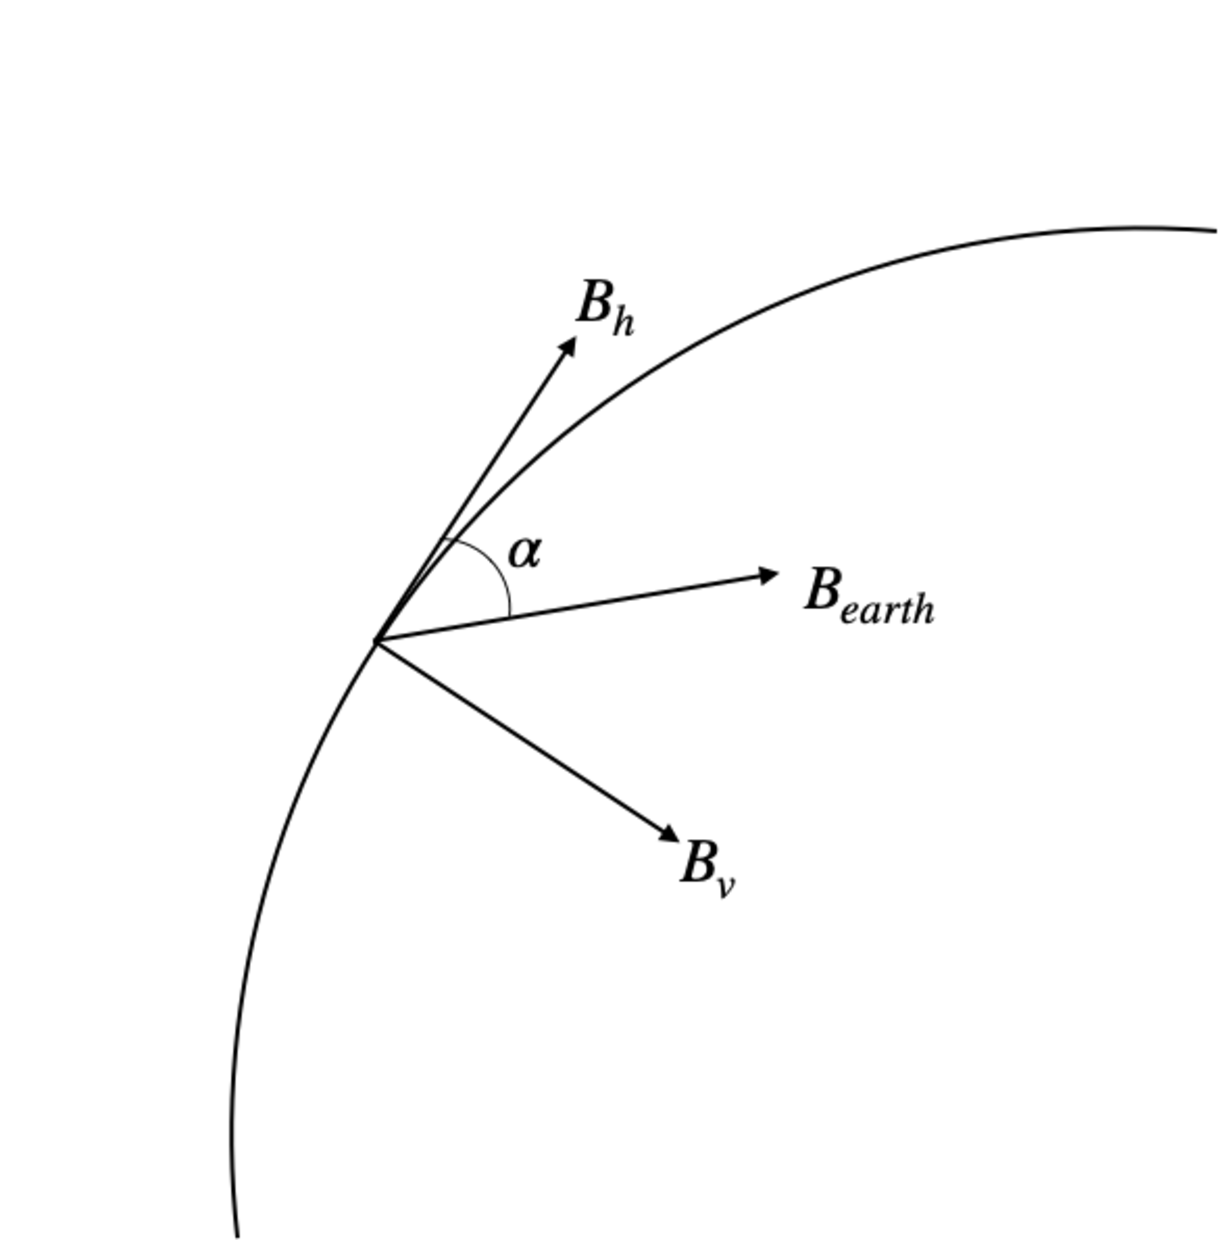
\includegraphics[width=3cm]{figures/1.pdf} 
\end{center}	

The magnetic field of earth can be resolved into two components
\[
   B_H = B_{earth} cos \alpha
\]
\[
   B_v = B_{earth} sin \alpha
\]

\section{Magnetic fields due to currents}

\subsection{Magnetic force due to long straight wire}
\begin{minipage}{0.5\textwidth}
   \begin{center}
    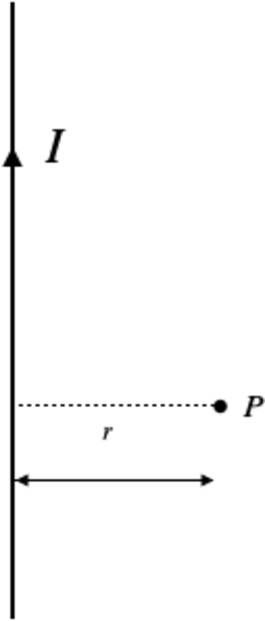
\includegraphics[width=2cm]{figures/3.pdf} 
   \end{center}	
\end{minipage}	
\begin{minipage}{0.5\textwidth}
\begin{itemize}
   \item the diretion of magnetic field is given by \textbf{Maxwell's right-hand grip rule}
   \item at point $P$, a distance $r$  away from the conductor, $B$ is given by
      \[
      B = \frac{\mu_0 I}{2 \pi r}
      \]
      where $\mu_0 = 4 \pi \times 10^{-7} Hm^{-1}$ 
      
\end{itemize}	
\end{minipage}	

\subsection{Magnetic fields due to circular coil}
\begin{minipage}{0.5\textwidth}
   \begin{center}
     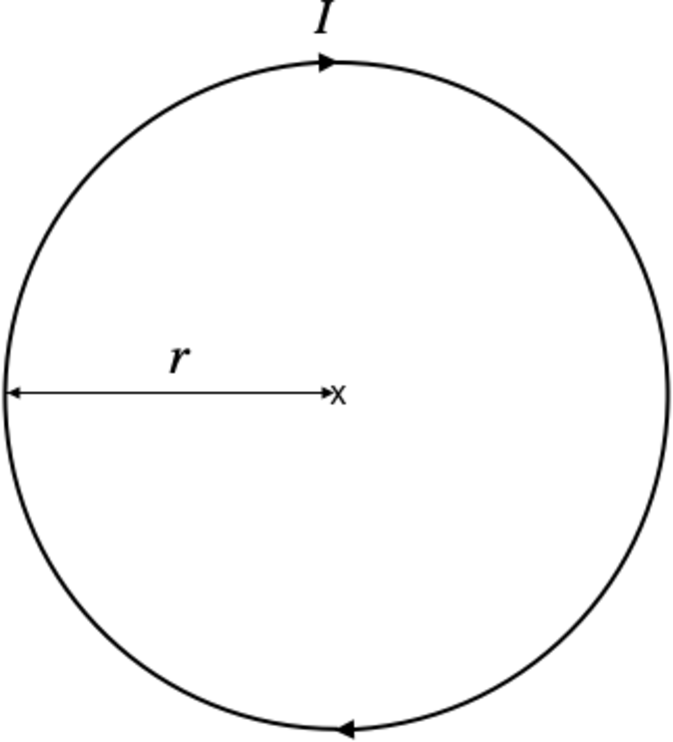
\includegraphics[width=3cm]{figures/4.pdf} 
   \end{center}	
\end{minipage}	
\begin{minipage}{0.5\textwidth}
   \begin{itemize}
      \item direction given by right-hand grip rule
      \item the magnetic flux density at the center of the coil is given by
         \[
         B = \frac{\mu_0 N I}{2r}
         \]
   \end{itemize}	
\end{minipage}	

\subsection{Magnetic field due to solenoid}

\begin{itemize}
   \item direction given by right-hand grip rule
   \item the magnetic flux density at the center of the solenoid is given by
      \[
      B = \mu_0 n I 
      \]
   \item the magnetic flux density at either end is
      \[
      B = \frac{1}{2} \mu_0 n I
      \]
   where $n$ is the number of turns per unit length
      
\end{itemize}	


\section{Force on a current carrying conductor}
\begin{framed}
The directions of current, field and force are given by \textbf{Fleming's left-hand rule}
\begin{center}
   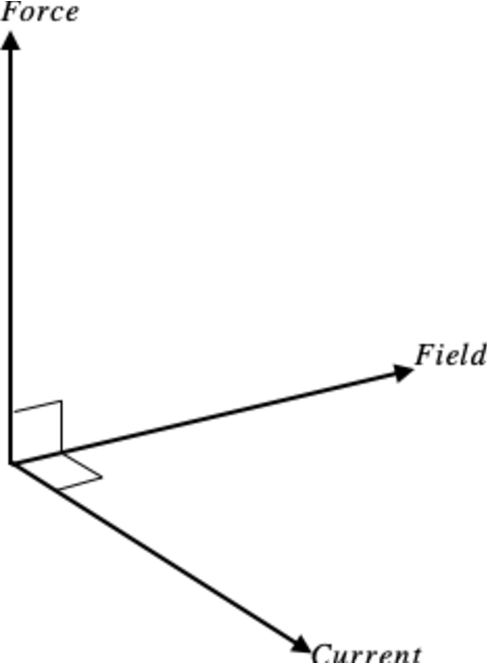
\includegraphics[width=3cm]{figures/2.pdf} 
\end{center}	
\end{framed}	

\subsection{Magnetic flux density, B}
\begin{framed}
   the \textbf{magnetic flux density} of a magnetic field is numerically equal to the \textbf{force per unit length} of a long straight conductor carrying a unit current at right angle to a uniform magnetic field
   \[
   B = \frac{F}{IL}
   \]
   hence,
   \[
   F = BIL
   \]
   

   For case in which magnetic field is at an angle $\theta$ to the current, the force on conductor is given by
   \[
   F = BIL sin \theta
   \]
   

   the S.I. unit is tesla \\
   one tesla is the uniform magnetic flux density which, acting normally to a long straight wire carrying a current of $1A$, causes a force per unit legnth of $1Nm^{-1}$ 
\end{framed}	

\subsection{Measuring magnetic flux density with a current balance}
\begin{center}
   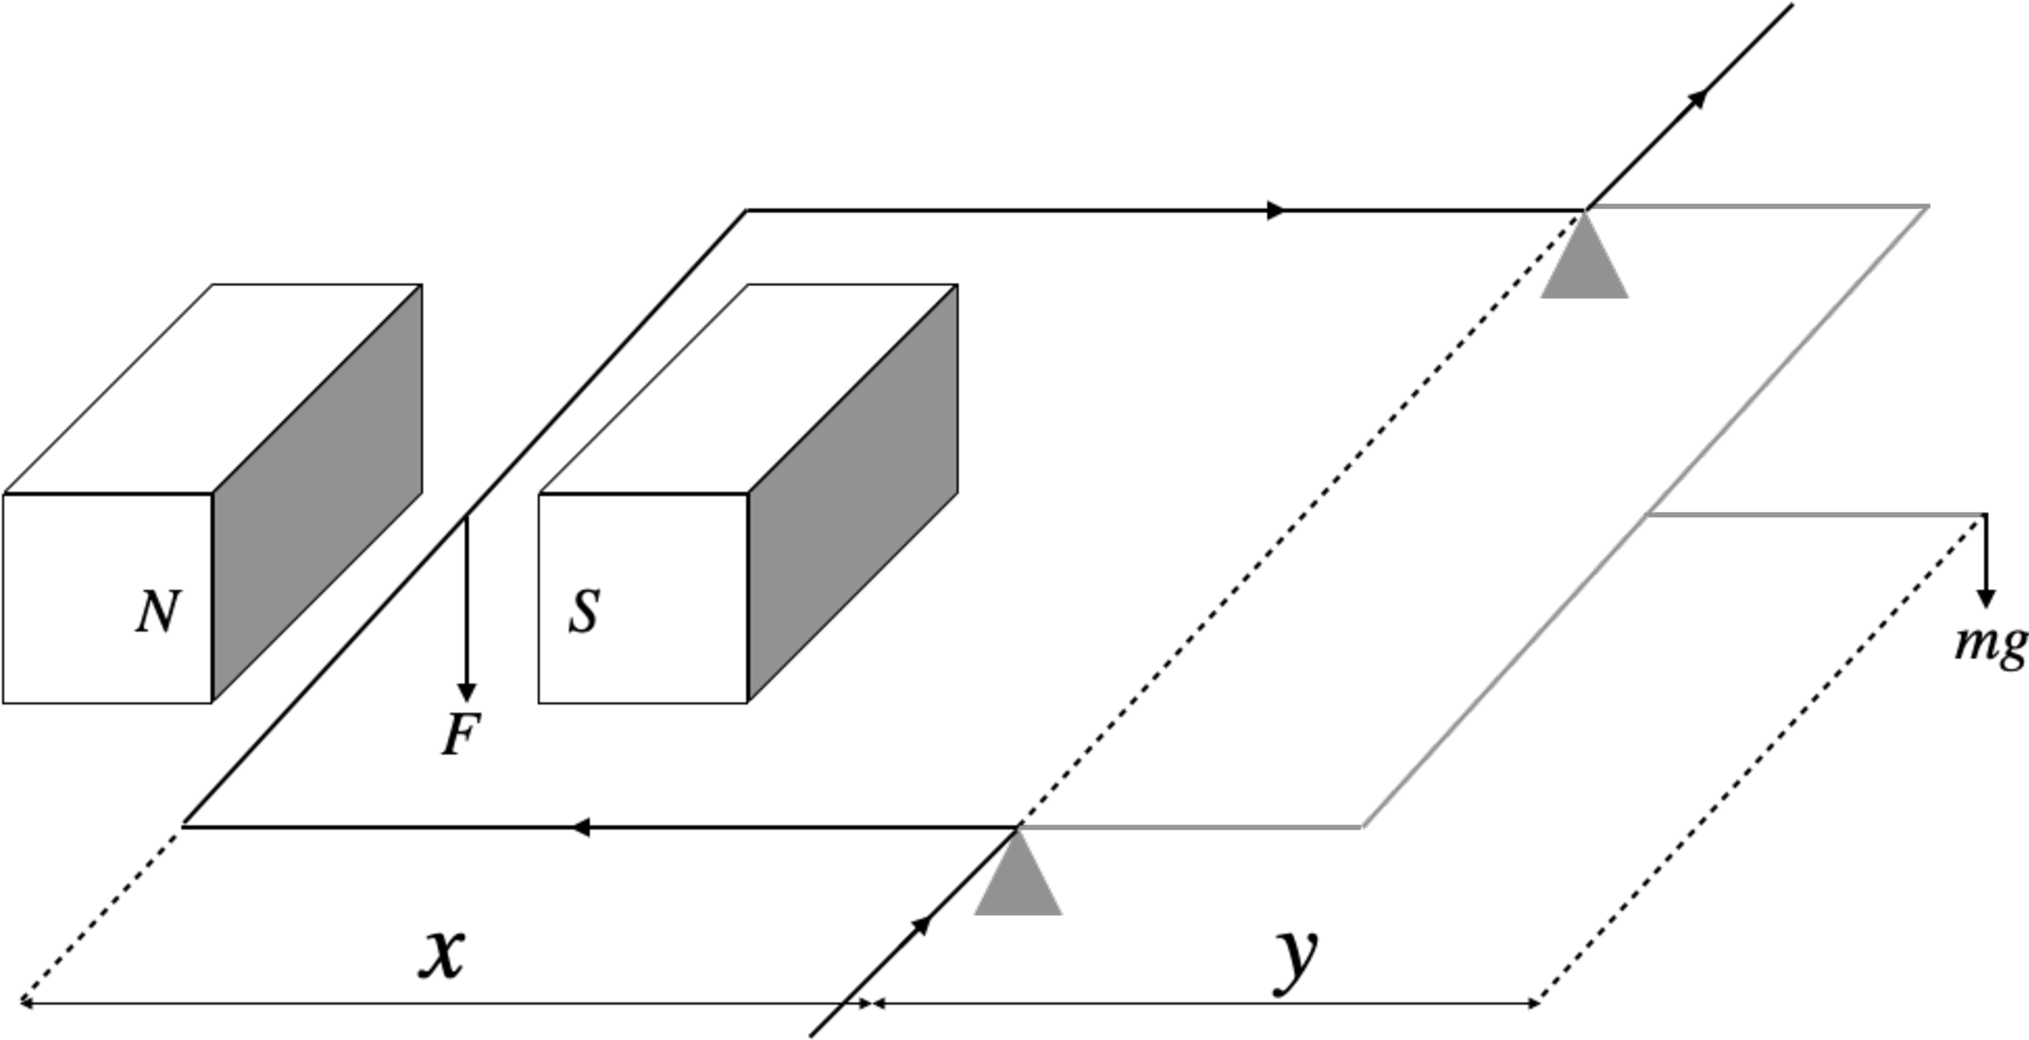
\includegraphics[width=3in]{figures/5.pdf} 
\end{center}	

By principle of moments, 
\[
   \text{sum of CW moments} =  \text{sum of ACW moments}
\]
\[
mgy = BILx
\]
\[
B = \frac{mgy}{ILx}
\]

\subsection{torque on current carrying coil in a magnetic field}
\begin{center}
   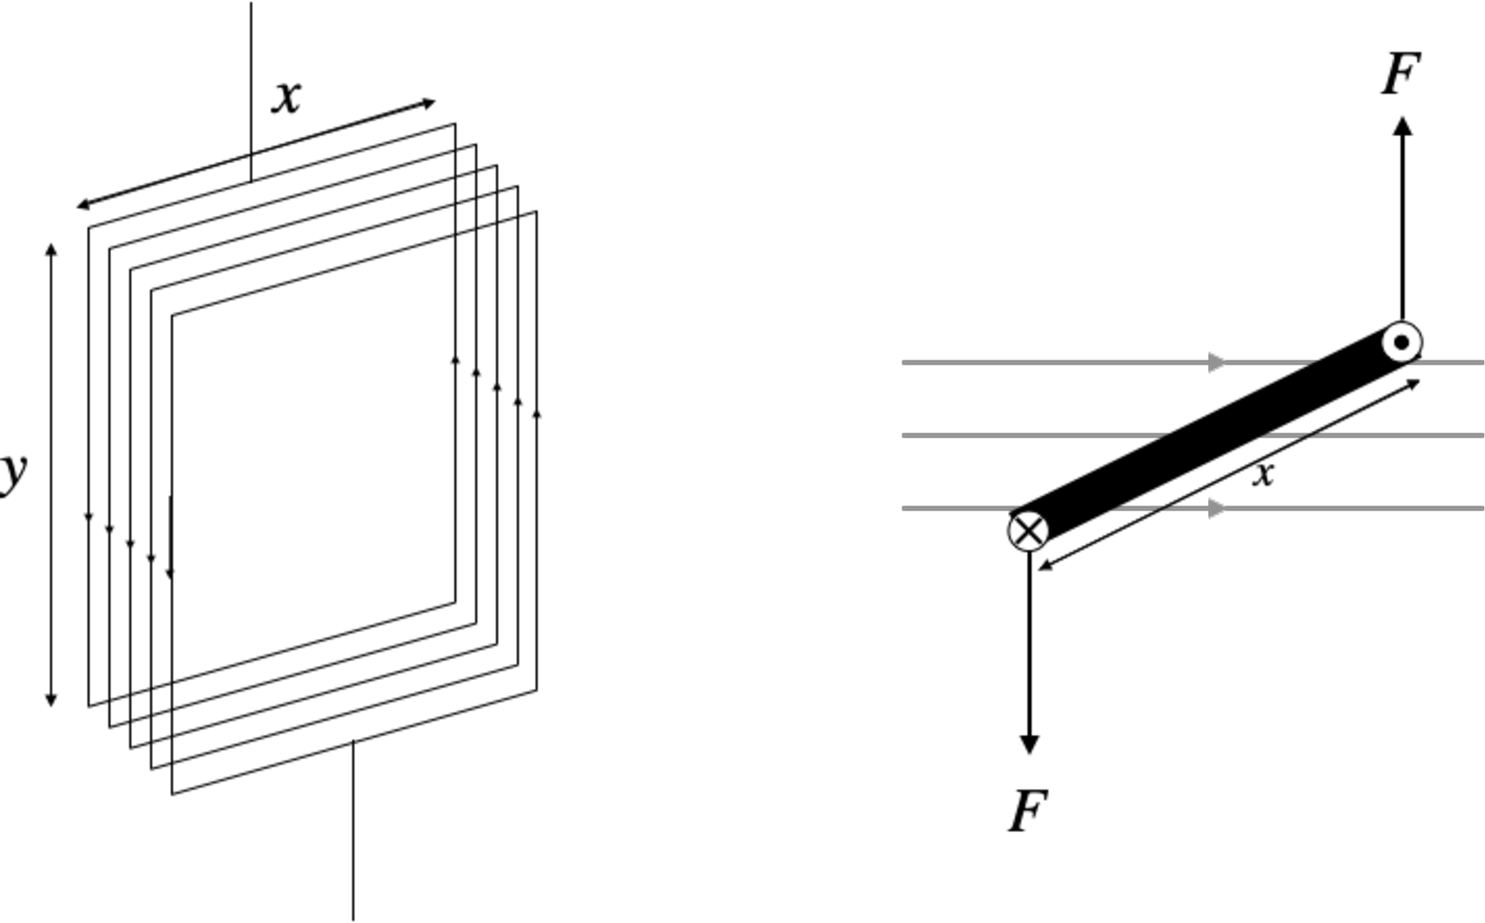
\includegraphics[width=3in]{figures/6.pdf} 
\end{center}	
\begin{itemize}
   \item the forces on vertical sides give rise to turning effect. the magnitude of each force is given by
      \[
      F = NBIy
      \]
   \item since the force on each vertical side are \textbf{equal in magnitude} and \textbf{opposite in direction}, the constitute a couple.
   \item the force on the vertical sides remain \textbf{constant in magnitude} throughout the rotation
   \item the torque of a couple is given by
      \[
      \tau = Fd
      \]
     where $d$ is the perpendicular distance between the lines of action of the forces
   \item the torque $\tau$ due to the conducting coil is thus
     \begin{align*}
        \tau &= Fd \\
             &= NBIy \times x cos \theta \\
             &= NBIyxcos \theta \\
             &= NBIA cos \theta
     \end{align*}	 
\end{itemize}	

\section{Force between current-carrying conductor}

\begin{center}
   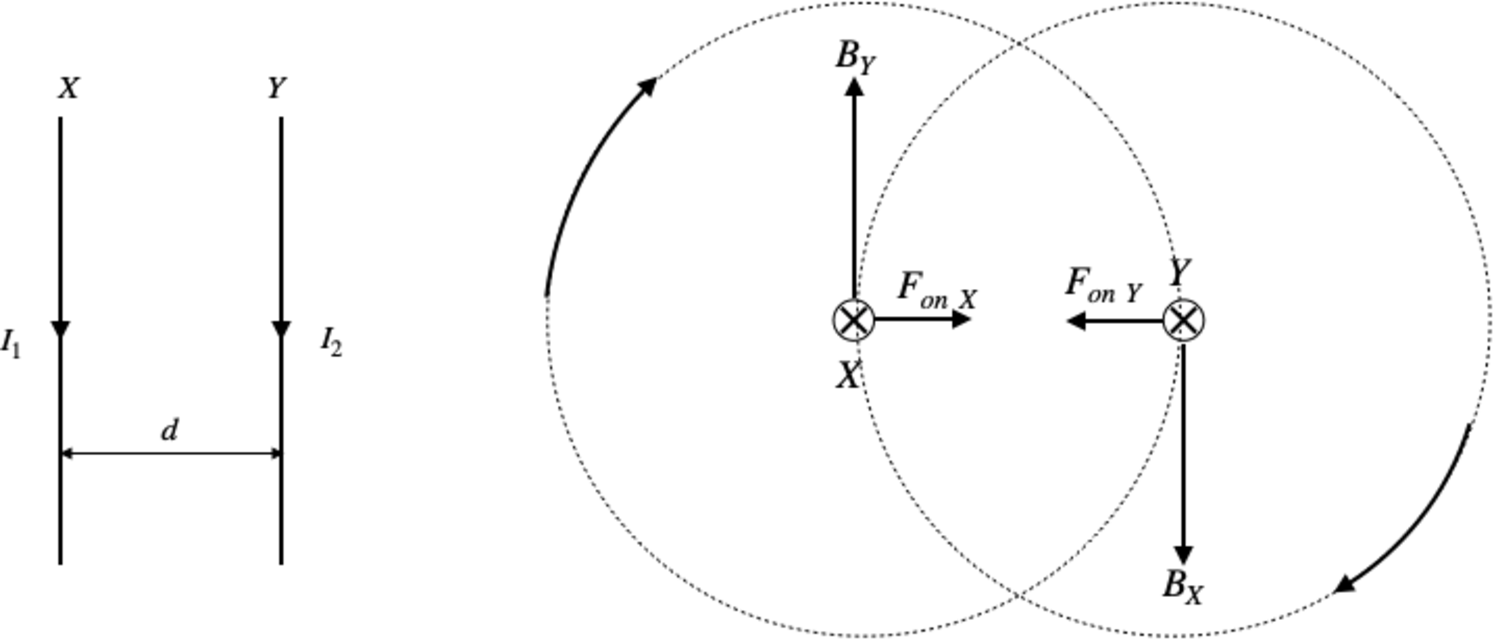
\includegraphics[width=3in]{figures/7.pdf} 
\end{center}	

The current in $X$ produces a magnetic field $B_X$, whose magnitude at $Y$ is given by
\[
   B_X = \frac{\mu_0 I_1}{2\pi d}
\]

Wire $Y$  thus experiences a magnetic force \textbf{towards X} and its magnitude is given by
\[
   F_{X on Y} = B_X I_2 L = \left( \frac{\mu_0 I_1}{2 \pi d} \right) I_2 L
\]
Likewise, X experiences a force \textbf{towards Y}, given by
\[
   F_{Y on X} = B_Y I_1 L = \left( \frac{\mu_0 I_2}{2 \pi d} \right) I_1 L
\]

The two wires with currents in the same direction \textbf{attract} each other, and the \textbf{force per unit length} on each wire is
\[
\frac{ F}{L} = \frac{\mu_0 I_1 I_2}{2 \pi d}
\]

In general
\begin{framed}
   For 2 parallel current-carrying conductors
   \begin{itemize}
      \item the force per unit length is 
         \[
         \frac{F}{L} = \frac{\mu_0 I_1 I_2}{2 \pi d}
         \]
      \item currents in the same direction attract, current in opposite directions repel
   \end{itemize}	
\end{framed}	

\section{Force on moving charge}

\begin{framed}
   For a charged particle travelling distance $L$ in time $t$, 
   \[
   v = \frac{L}{t}
   \]
   The moving charge constitutes a current where 
   \[
      I = \frac{q}{t}
   \]
   Hence force on charge is given by 
   \[
      F = BIL = \left( \frac{BqL}{t} \right) = Bqv
   \]

   If velocity and field are inclined to each other by angle $\theta$, 
   \[
   F = Bqv sin \theta
   \]

   Note that direction of current is that of \textbf{conventional current}
\end{framed}	

\subsection{Motion of charged particle in magnetic field}
For a charged particle projected at right angle into a magnetic field \\
\begin{minipage}{0.5\textwidth}
   \begin{center}
      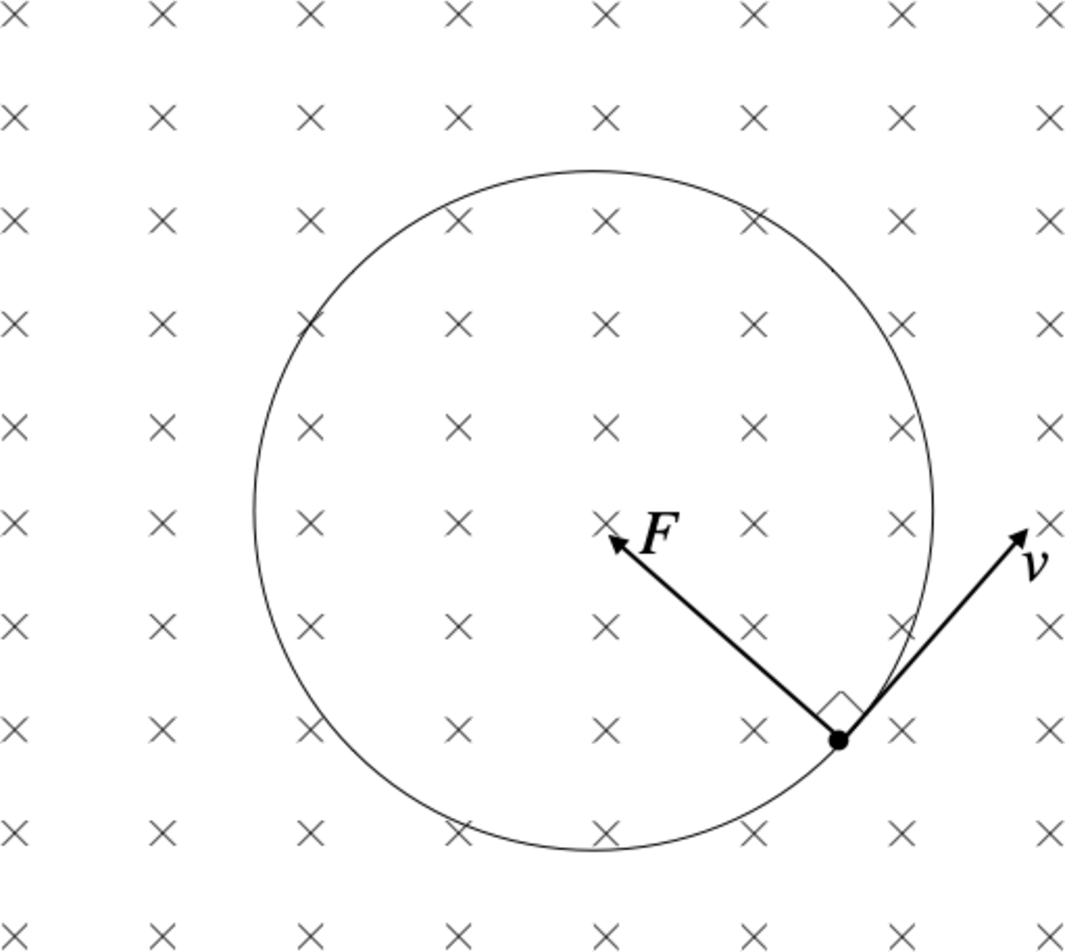
\includegraphics[width=5cm]{figures/8.pdf} 
   \end{center}	
\end{minipage}
\begin{minipage}{0.5\textwidth}
   the \textbf{magnetic force} on moving charge provides for centripetal force
   \[
      Bqv = \frac{mv^2}{2}
   \]
\end{minipage}

For a charged particle projected at some angle $\theta$, 
\[
   v_{parallel} = v\ cos\theta
\]
\[
   v_{perpendicular} = v\ sin \theta
\]


\section{the velocity selector}
\begin{center}
   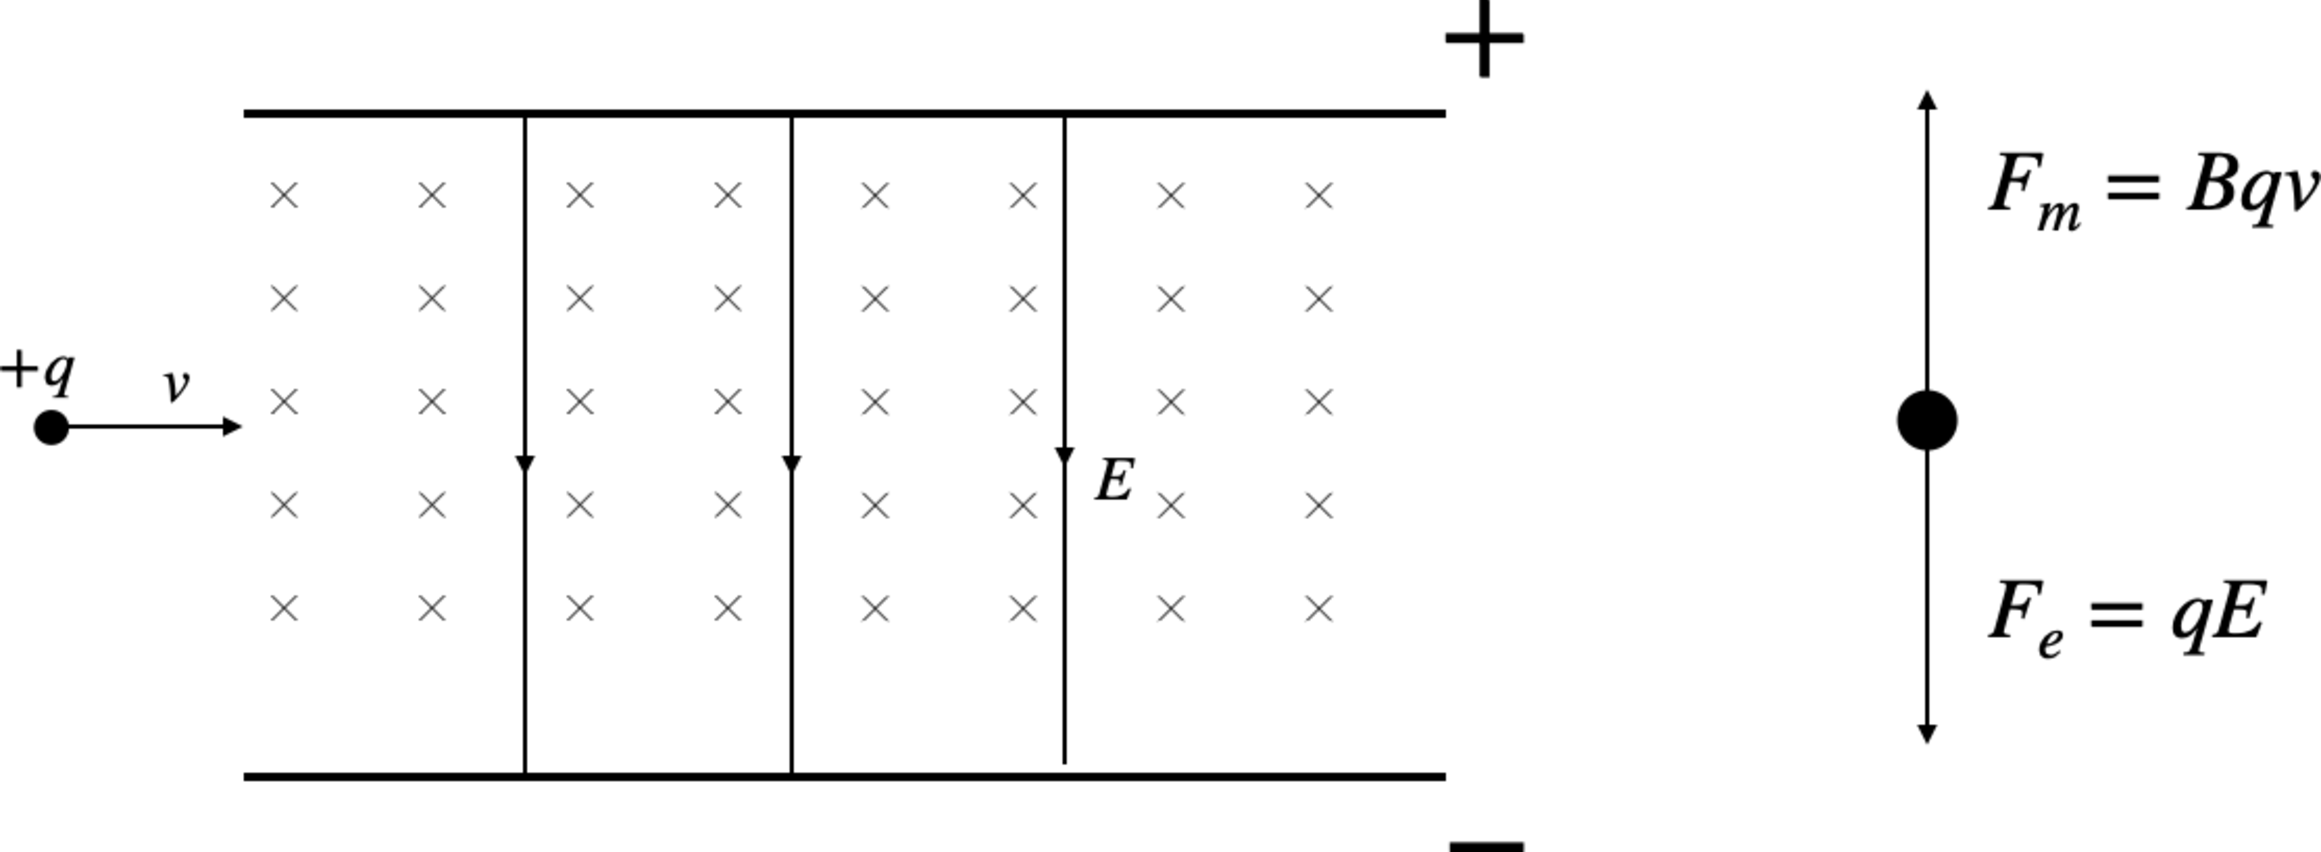
\includegraphics[width=3in]{figures/9.pdf} 
\end{center}	
Particles deflect upwards or downwards depending on $F_m$ and $F_e$

Particles experience no deflection when
\[
Bqv = qE
\]
\[
v = \frac{E}{B}
\]



\end{document}	
